\documentclass[10pt]{beamer}
\usepackage{graphicx}
\usepackage{tikz}
\usepackage{lmodern}
\usepackage{mathtools}
\usepackage{amsmath,bm}
\usepackage{minted}
\usepackage[backend=bibtex]{biblatex}
\usepackage{hyperref}
\usepackage{multirow}
\usetheme{CambridgeUS}
\usecolortheme{seahorse}
\setbeamercovered{dynamic}
\usefonttheme{professionalfonts}
\setbeamertemplate{itemize items}[default]
\setbeamerfont{caption}{size=\footnotesize}
\addbibresource{bibliography.bib}
\setcounter{tocdepth}{2}
\newcommand*{\Scale}[2][4]{\scalebox{#1}{$#2$}}%
\newcommand*{\Resize}[2]{\resizebox{#1}{!}{$#2$}}%

\begin{document}

\begin{frame}{Fourth order Pade scheme}
\begin{itemize}
\item{Inner grid points:
\begin{align*}
f_i^{\prime} + \frac{1}{4}(f^{\prime}_{i-1} + f^{\prime}_{i+1}) = \
\frac{3}{4}\frac{f_{i+1} - f_{i-1}}{dx}
\end{align*}}

\item{Boundary points:
\begin{align*}
f^{\prime}_1 + 2f^{\prime}_2 &= \frac{-5f_1 + 4f_2 + f_3}{dx} \\
%
f^{\prime}_{n} + 2f^{\prime}_{n-1}
&=
\frac{5f_{n} - 4f_{n-2} -  f_{n-1}}{dx}
\end{align*}}
\end{itemize}
\end{frame}

\begin{frame}
\frametitle{Kernels and thread organization}
\begin{columns}
\begin{column}{0.5\textwidth}
\textbf{Kernels}
\begin{itemize}
\item Special pieces of code that execute on the GPU
\item In Fortran: subroutines; in C: functions
\item Executed concurrently by several GPU threads
\end{itemize}
\textbf{Threads}
\begin{itemize}
\item Threads organized into a grid of blocks
\item Kernels launched with specified grid size
    (number of blocks) and block size (threads per block)
\item Grid and blocks can be 2-D or 3-D for convenience
\end{itemize}
\end{column}
\begin{column}{0.5\textwidth}
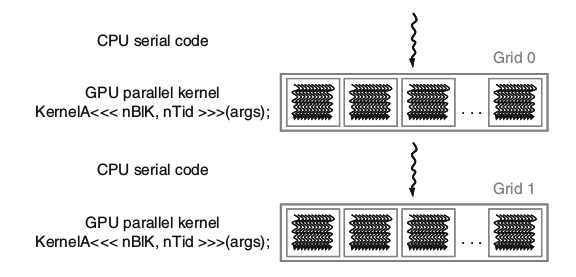
\includegraphics[width=120px]{img/program-structure.png}
\vspace{1cm}
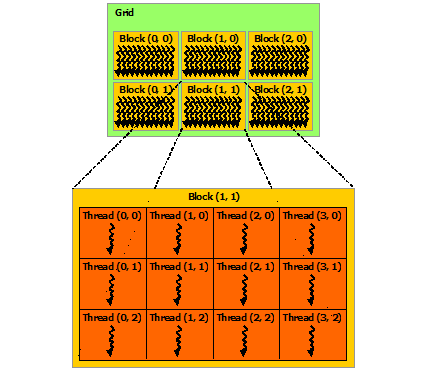
\includegraphics[width=120px]{img/grid-of-thread-blocks.png}
\end{column}
\end{columns}
\end{frame}

\begin{frame}
\frametitle{GPU Architecture}
\begin{columns}
\begin{column}{0.5\textwidth}
\begin{itemize}
\item GPU viewed as a collection of \emph{streaming microprocessors} (SMs)
\item When kernel is launched, each block gets assigned to an SM
\item Threads within a block execute concurrently
\item SM may execute several blocks concurrently
\end{itemize}
\end{column}
\begin{column}{0.5\textwidth}
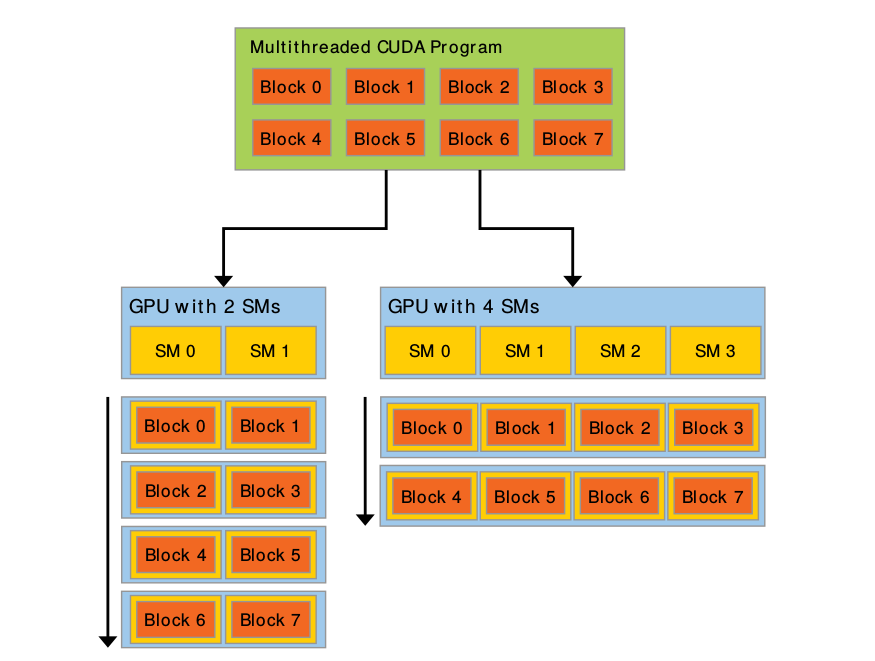
\includegraphics[width=150px]{img/gpu-scaling.png}
\end{column}
\end{columns}
\end{frame}

\begin{frame}
\frametitle{Memory hierarchy}
\begin{columns}
\begin{column}{0.5\textwidth}
\begin{itemize}
\item Global memory{
\begin{itemize}
    \item large but slow (~5 GB for Tesla K20)
    \item CPU can access (via PCI-e bus)
    \item all threads can access
    \item persists between kernel launches
\end{itemize}}
\item Shared memory{
\begin{itemize}
    \item small but fast (~48 KiB per SM and block)
    \item local to threads within a block
    \item threads in a block read and write into shared memory
    \item explicitly managed cache
\end{itemize}}
\item Registers{
\begin{itemize}
    \item limited (65536 per SM and block)
    \item local to individual threads
    \item fastest
\end{itemize}}
\end{itemize}
\end{column}
\begin{column}{0.5\textwidth}
    \visible{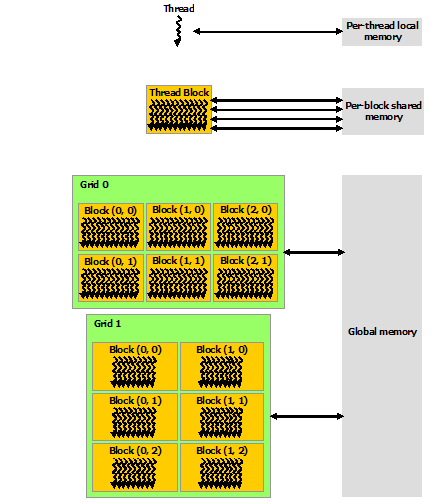
\includegraphics[width=150px]{img/memory-hierarchy.png}}
\end{column}
\end{columns}
\end{frame}

\begin{frame}
\frametitle{GPU implementation}
\begin{columns}
\begin{column}{0.5\textwidth}
\begin{itemize}
\item Each tridiagonal system mapped to a thread block;
    individual threads mapped to equations
\item Several systems can be solved at concurrently
\item Forward reduction: diagonal arrays $a$, $b$, $c$ and RHS $d$
    updated \emph{in-place}
\item Backward substitution: solution $x$ computed
    from $a^\prime$, $b^\prime$, $c^\prime$ and $d^\prime$
\item Synchronization required at each step
\end{itemize}
\end{column}
\begin{column}{0.5\textwidth}
\only<1>{
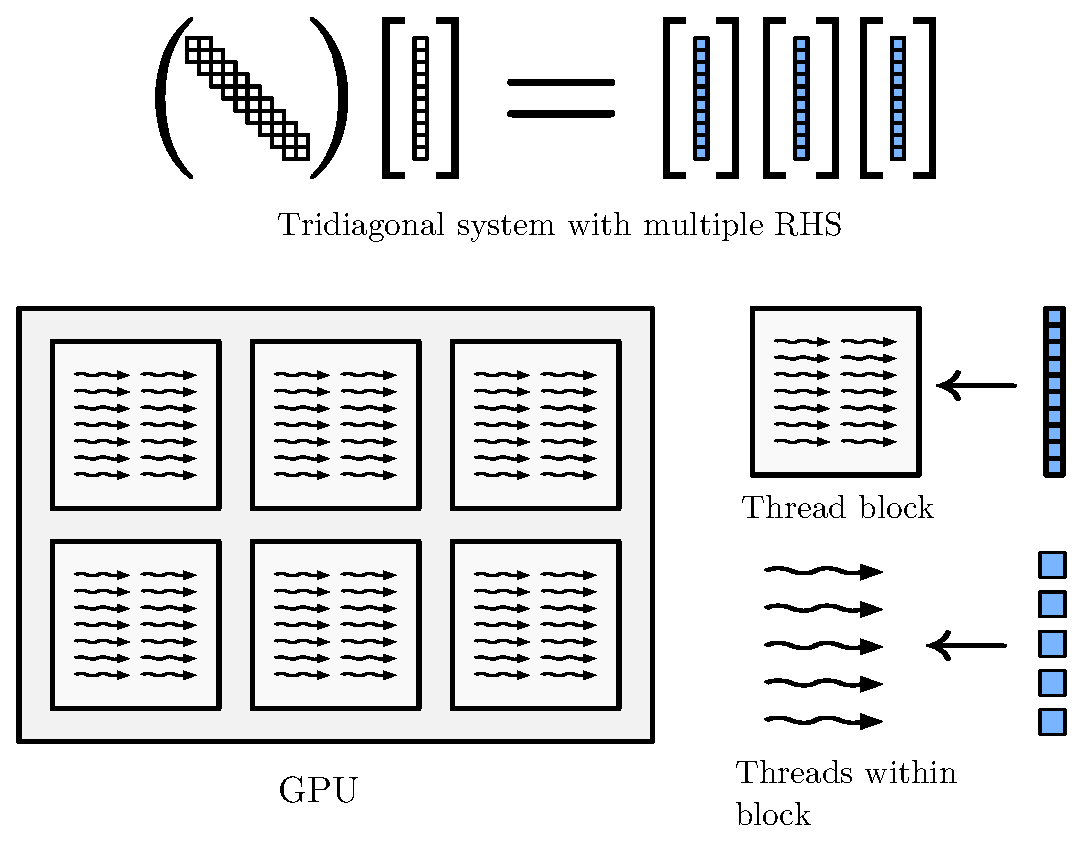
\includegraphics[width=150px]{img/gpu-mapping.eps}
}
\only<2>{
\centering
Forward reduction
\scalebox{0.8}{
\vbox{
\begin{align*} 
    k_1 &= \frac{a_i}{b_{i-1}}, k_2 = \frac{c_i}{b_{i+1}} \\
    a^{\prime}_i &= -a_{i-1}k_1 \\
    b^{\prime}_i &= b_i - c_{i-1}k_1 - a_{i+1}k_2 \\
    c^{\prime}_i &= -c_{i+1}k_2 \\
    d^{\prime}_i &= d_i - d_{i-1}k_1  - d_{i+1}k_2 \\
\end{align*}}}

\centering
Backward substitution
\scalebox{0.8}{
\vbox{
\begin{align*}
x_i &= \frac{d^{\prime}_i - a^{\prime}_ix_{i-1} - \
    c^{\prime}_ix_{i+1}}{b^{\prime}_i}
\end{align*}}}}

\end{column}
\end{columns}
\end{frame}

